% Copyright 2004 by Till Tantau <tantau@users.sourceforge.net>.
%
% In principle, this file can be redistributed and/or modified under
% the terms of the GNU Public License, version 2.
%
% However, this file is supposed to be a template to be modified
% for your own needs. For this reason, if you use this file as a
% template and not specifically distribute it as part of a another
% package/program, I grant the extra permission to freely copy and
% modify this file as you see fit and even to delete this copyright
% notice. 

\documentclass{beamer}

\usepackage{blindtext}
\usepackage{tcolorbox}

\usefonttheme{professionalfonts} % using non standard fonts for beamer
\usefonttheme{serif} % default family is serif
%\usepackage{fontspec}
%\setmainfont{Liberation Serif}

% There are many different themes available for Beamer. A comprehensive
% list with examples is given here:
% http://deic.uab.es/~iblanes/beamer_gallery/index_by_theme.html
% You can uncomment the themes below if you would like to use a different
% one:
%\usetheme{AnnArbor}
%\usetheme{Antibes}
%\usetheme{Bergen}
%\usetheme{Berkeley}
%\usetheme{Berlin}
%\usetheme{Boadilla}
%\usetheme{boxes}
%\usetheme{CambridgeUS}
%\usetheme{Copenhagen}
%\usetheme{Darmstadt}
\usetheme{default}
%\usetheme{Frankfurt}
%\usetheme{Goettingen}
%\usetheme{Hannover}
%\usetheme{Ilmenau}
%\usetheme{JuanLesPins}
%\usetheme{Luebeck}
%\usetheme{Madrid}
%\usetheme{Malmoe}
%\usetheme{Marburg}
%\usetheme{Montpellier}
%\usetheme{PaloAlto}
%\usetheme{Pittsburgh}
%\usetheme{Rochester}
%\usetheme{Singapore}
%\usetheme{Szeged}
%\usetheme{Warsaw}



\title{Digital Signal Processing: Theory and Practice}

% A subtitle is optional and this may be deleted
\subtitle{\textbf{Some useful and important signals}}

\author{Sivakumar Balasubramanian}
% - Give the names in the same order as the appear in the paper.
% - Use the \inst{?} command only if the authors have different
%   affiliation.

\institute[Christian Medical College] % (optional, but mostly needed)
{
  \inst{}%
  Department of Bioengineering\\
  Christian Medical College, Bagayam\\
  Vellore 632002
}
% - Use the \inst command only if there are several affiliations.
% - Keep it simple, no one is interested in your street address.

\date{}
% - Either use conference name or its abbreviation.
% - Not really informative to the audience, more for people (including
%   yourself) who are reading the slides online

\subject{Lecture notes on signal processing}
% This is only inserted into the PDF information catalog. Can be left
% out.

% If you have a file called "university-logo-filename.xxx", where xxx
% is a graphic format that can be processed by latex or pdflatex,
% resp., then you can add a logo as follows:

% \pgfdeclareimage[height=0.5cm]{university-logo}{university-logo-filename}
% \logo{\pgfuseimage{university-logo}}

% Delete this, if you do not want the table of contents to pop up at
% the beginning of each subsection:
\AtBeginSubsection[]
{
  \begin{frame}<beamer>{Outline}
    \tableofcontents[currentsection,currentsubsection]
  \end{frame}
}

% Let's get started
\begin{document}

\begin{frame}
  \titlepage
\end{frame}

% USEFUL SIGNALS IN CONTINUOUS AND DISCRETE TIME
\begin{frame}[t]{Useful discrete-time signals}

We will look at some important signals, that we will often come across and are useful in the analysis of signals and systems.
\begin{itemize}
\item Exponential signals
\item Sinusoids
\item Exponential sinusoids
\item Impulse function
\item Step function
\end{itemize}

\end{frame}

%% REAL EXPONENTIALS
%\begin{frame}[t]{Real Exponentials}
%
%\textbf{Continuous-time} version
%\[ x(t) = be^{at} \]
%
%where, $a, b, t \in \mathbb{R}$. $b$ is the amplitude and $a$ is the exponential growth or decay rate.
%
%\begin{figure}
%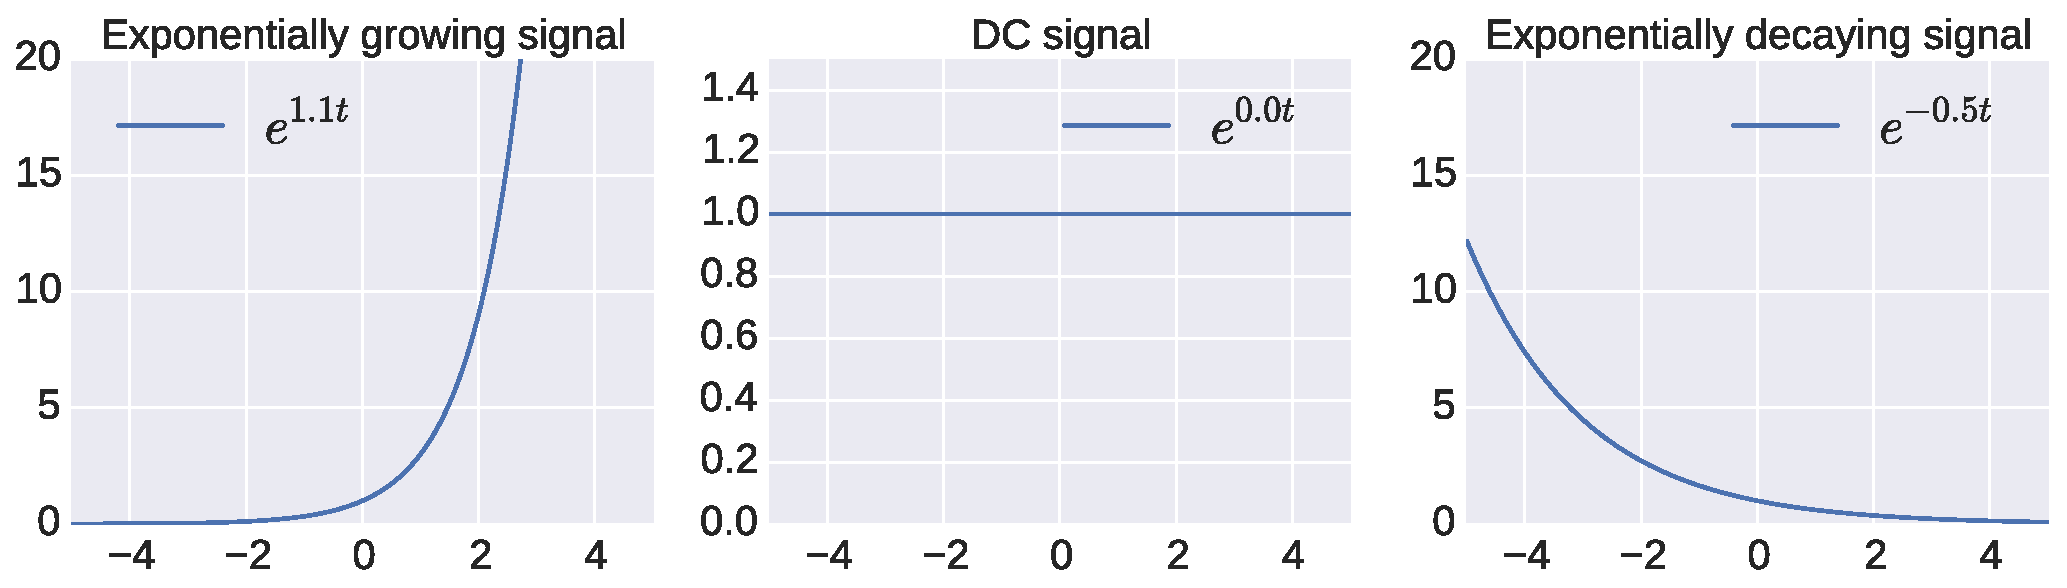
\includegraphics[width=\textwidth]{img/exp.eps}
%\end{figure}
%\end{frame}

% REAL EXPONENTIALS
\begin{frame}[t]{Real Exponentials}

\textbf{Discrete-time} version
\[ x[n] =  b \left(a\right)^n \]

where, $a, b \in \mathbb{R}$ and $n \in \mathbb{Z}$. $b$ is the amplitude and $a$ is the exponential growth or decay rate.

\begin{figure}
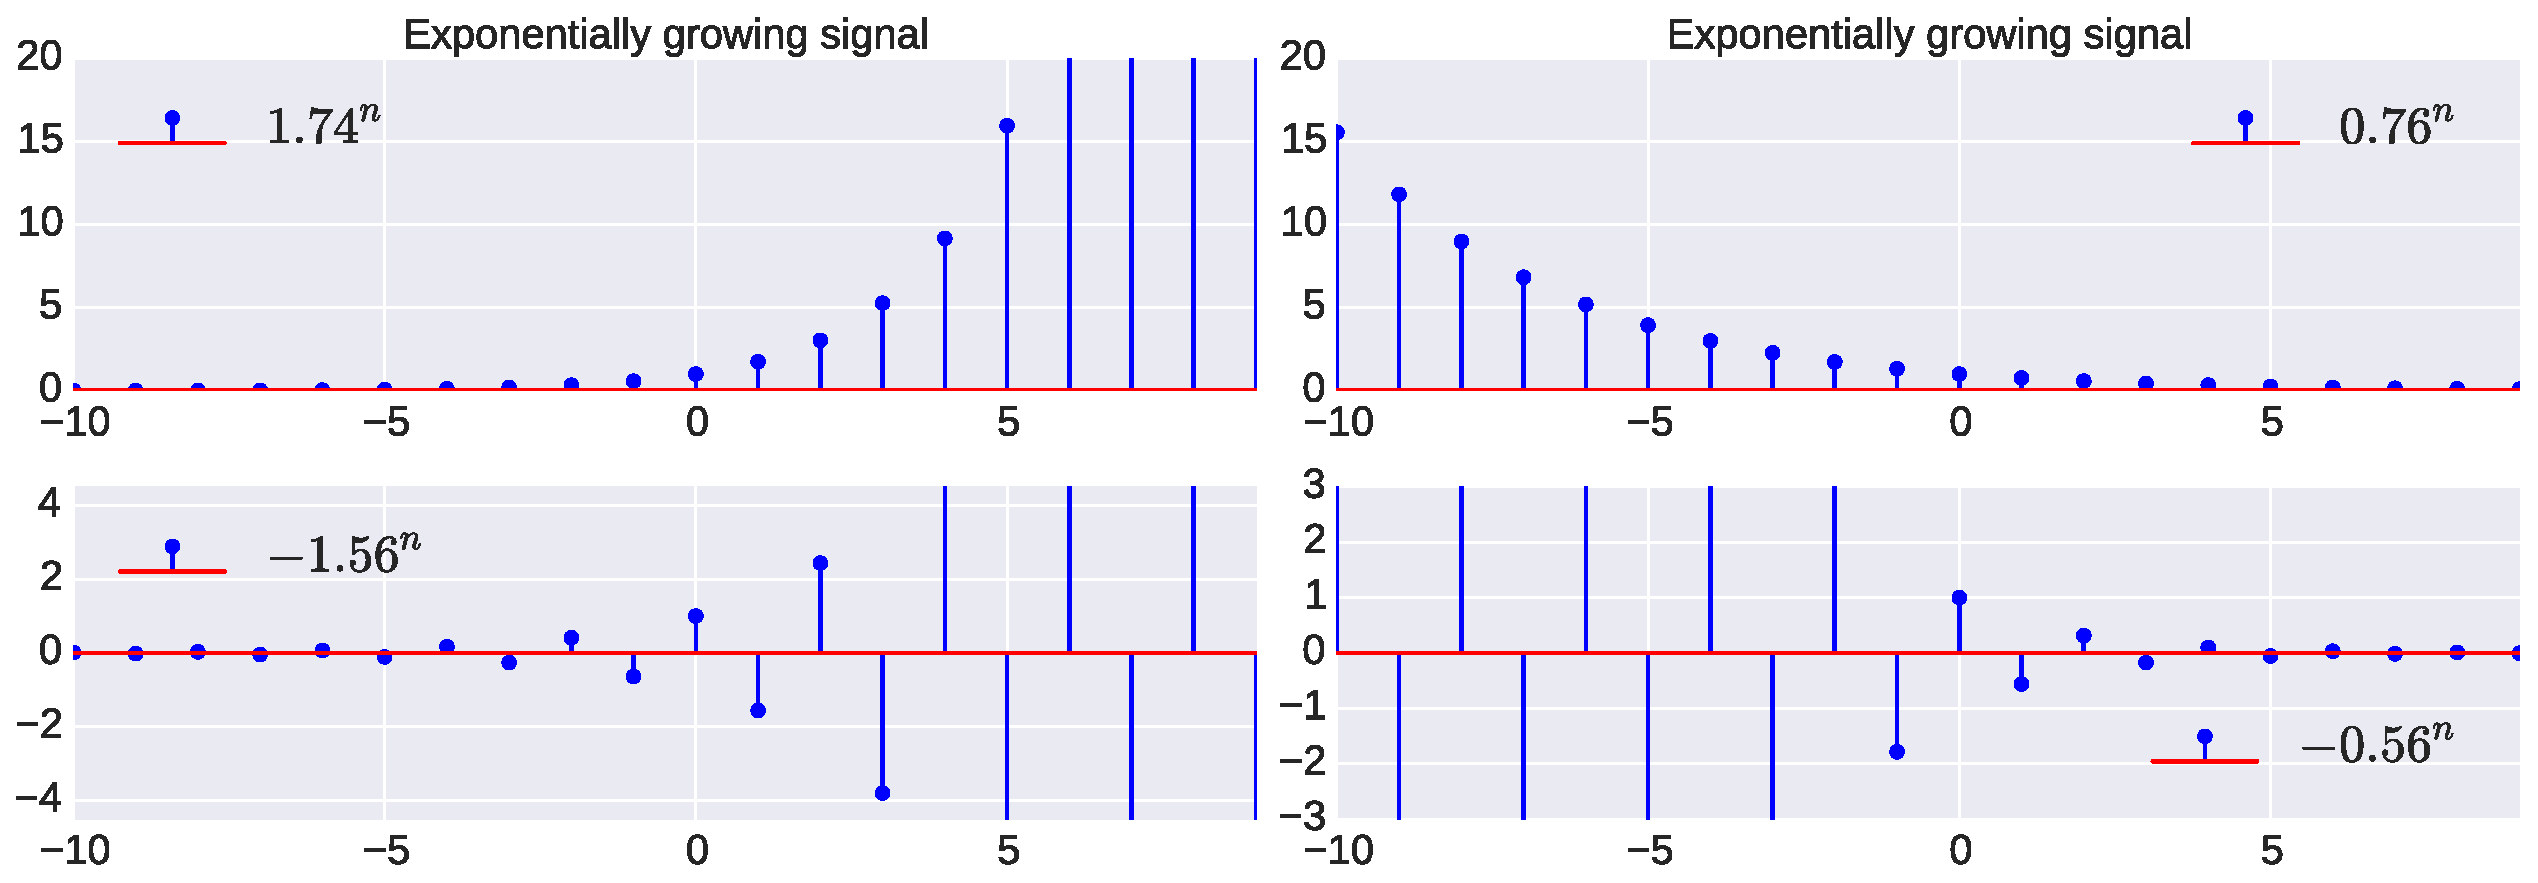
\includegraphics[width=\textwidth]{img/disc_exp.eps}
\end{figure}
\end{frame}

% REAL EXPONENTIALS
\begin{frame}[t]{Real Exponentials}

These are encountered as solution to first order difference equations.
%\[ \frac{d}{dt}x(t) = kx(t) \implies x(t) = Ce^{kt} \]
\[ x[n] = kx[n-1] \implies x(t) = C(k)^n \]

Can you think of practical examples of systems that result in such signals?
\end{frame}

% SINUSOIDAL SIGNALS
%\begin{frame}[t]{Sinusoidal signals}
%\textbf{Continuous-time} version
%
%\[ x(t) = A \sin \left(\omega t + \phi\right) \]
%
%where, $A$ is the amplitude, $\omega$ is the angular frequency $\left(\mathrm{rad}.\mathrm{sec}^{-1}\right)$, and $\phi$ is the phase angle.
%
%\begin{figure}
%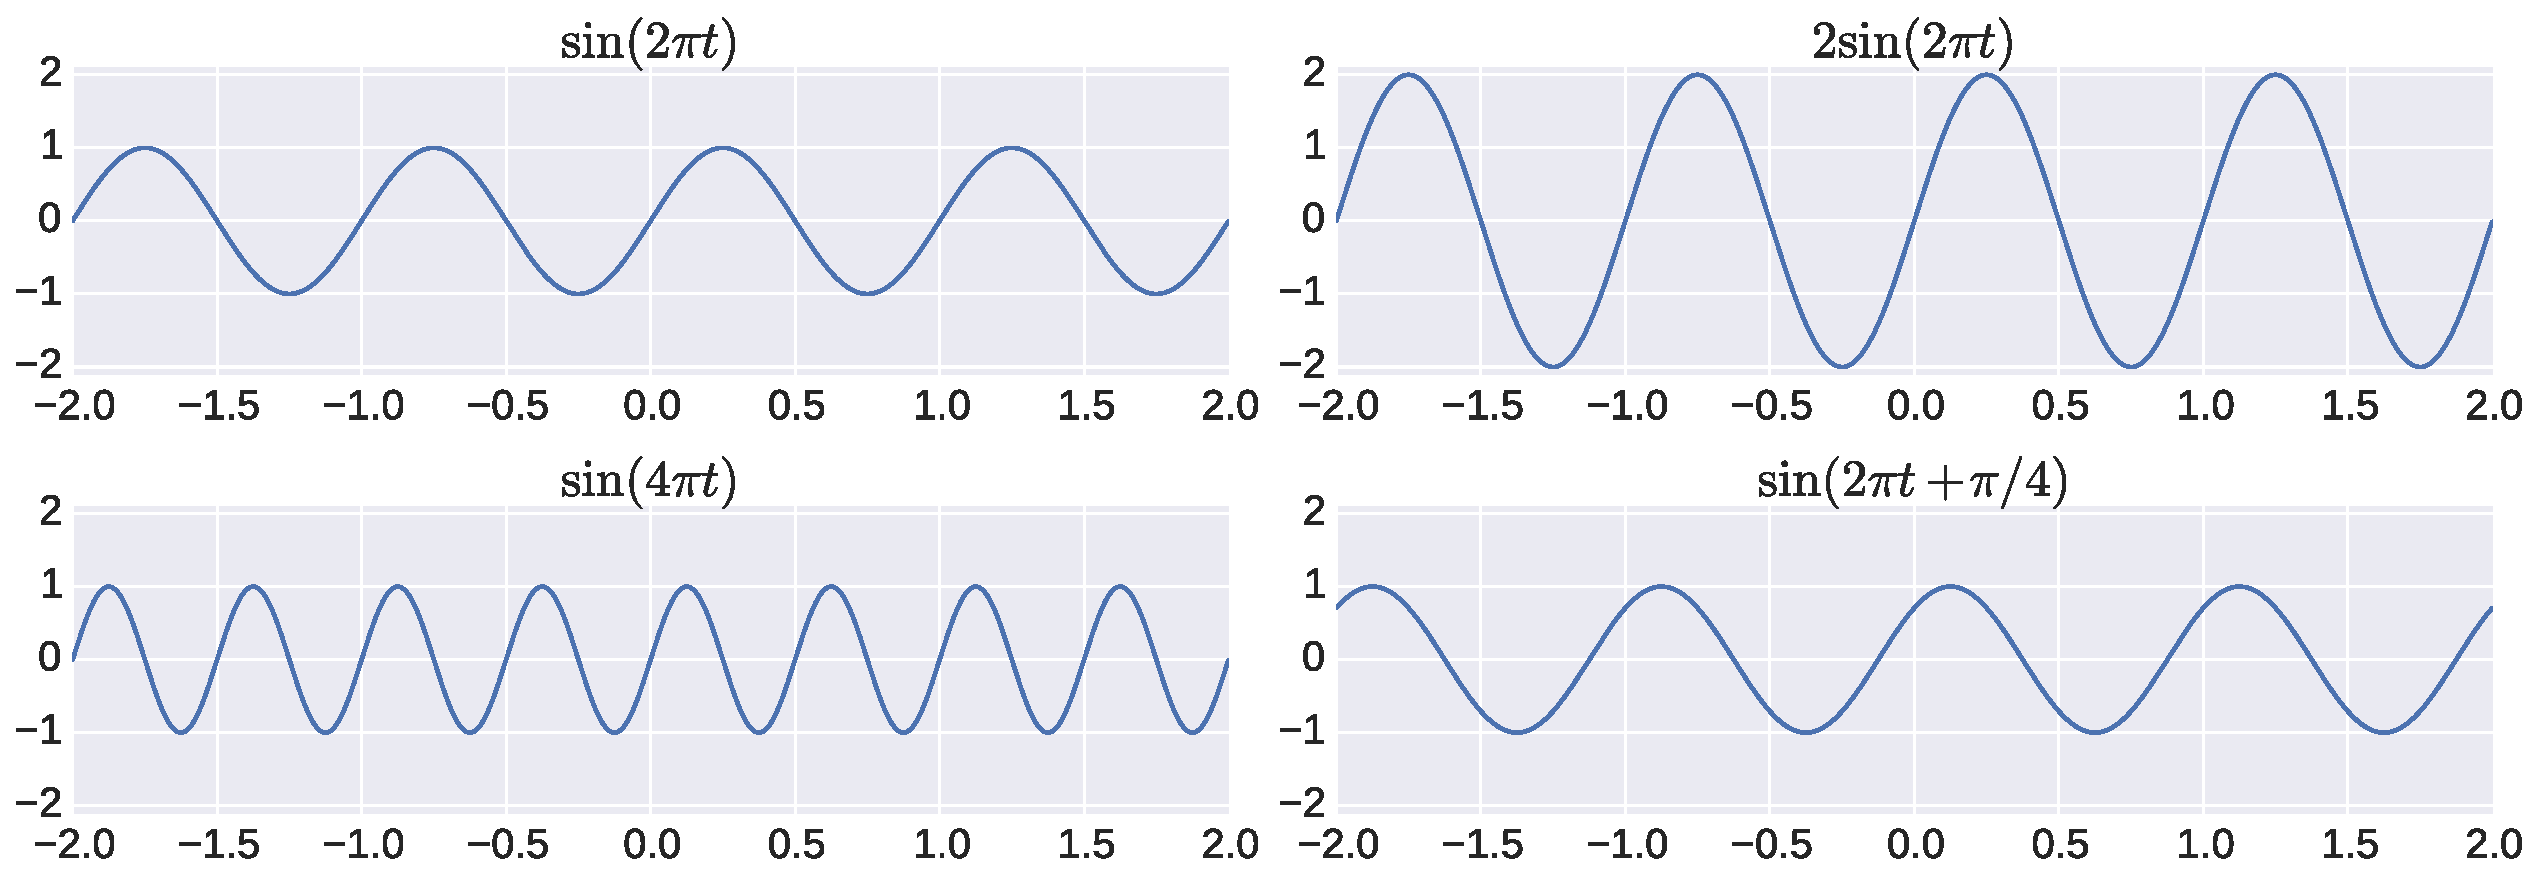
\includegraphics[width=\textwidth]{img/sinu.eps}
%\end{figure}
%
%What is the fundamental period of sinusoid?
%\end{frame}

% SINUSOIDAL SIGNALS
\begin{frame}[t]{Sinusoidal signals}
\textbf{Discrete-time} version

\[ x[n] = A \sin \left(\Omega n + \phi\right) \]

where, $A$ is the amplitude, $\Omega$ is the digital frequency $\left(\mathrm{rad}.\mathrm{sample}^{-1}\right)$, and $\phi$ is the phase angle.

\begin{figure}
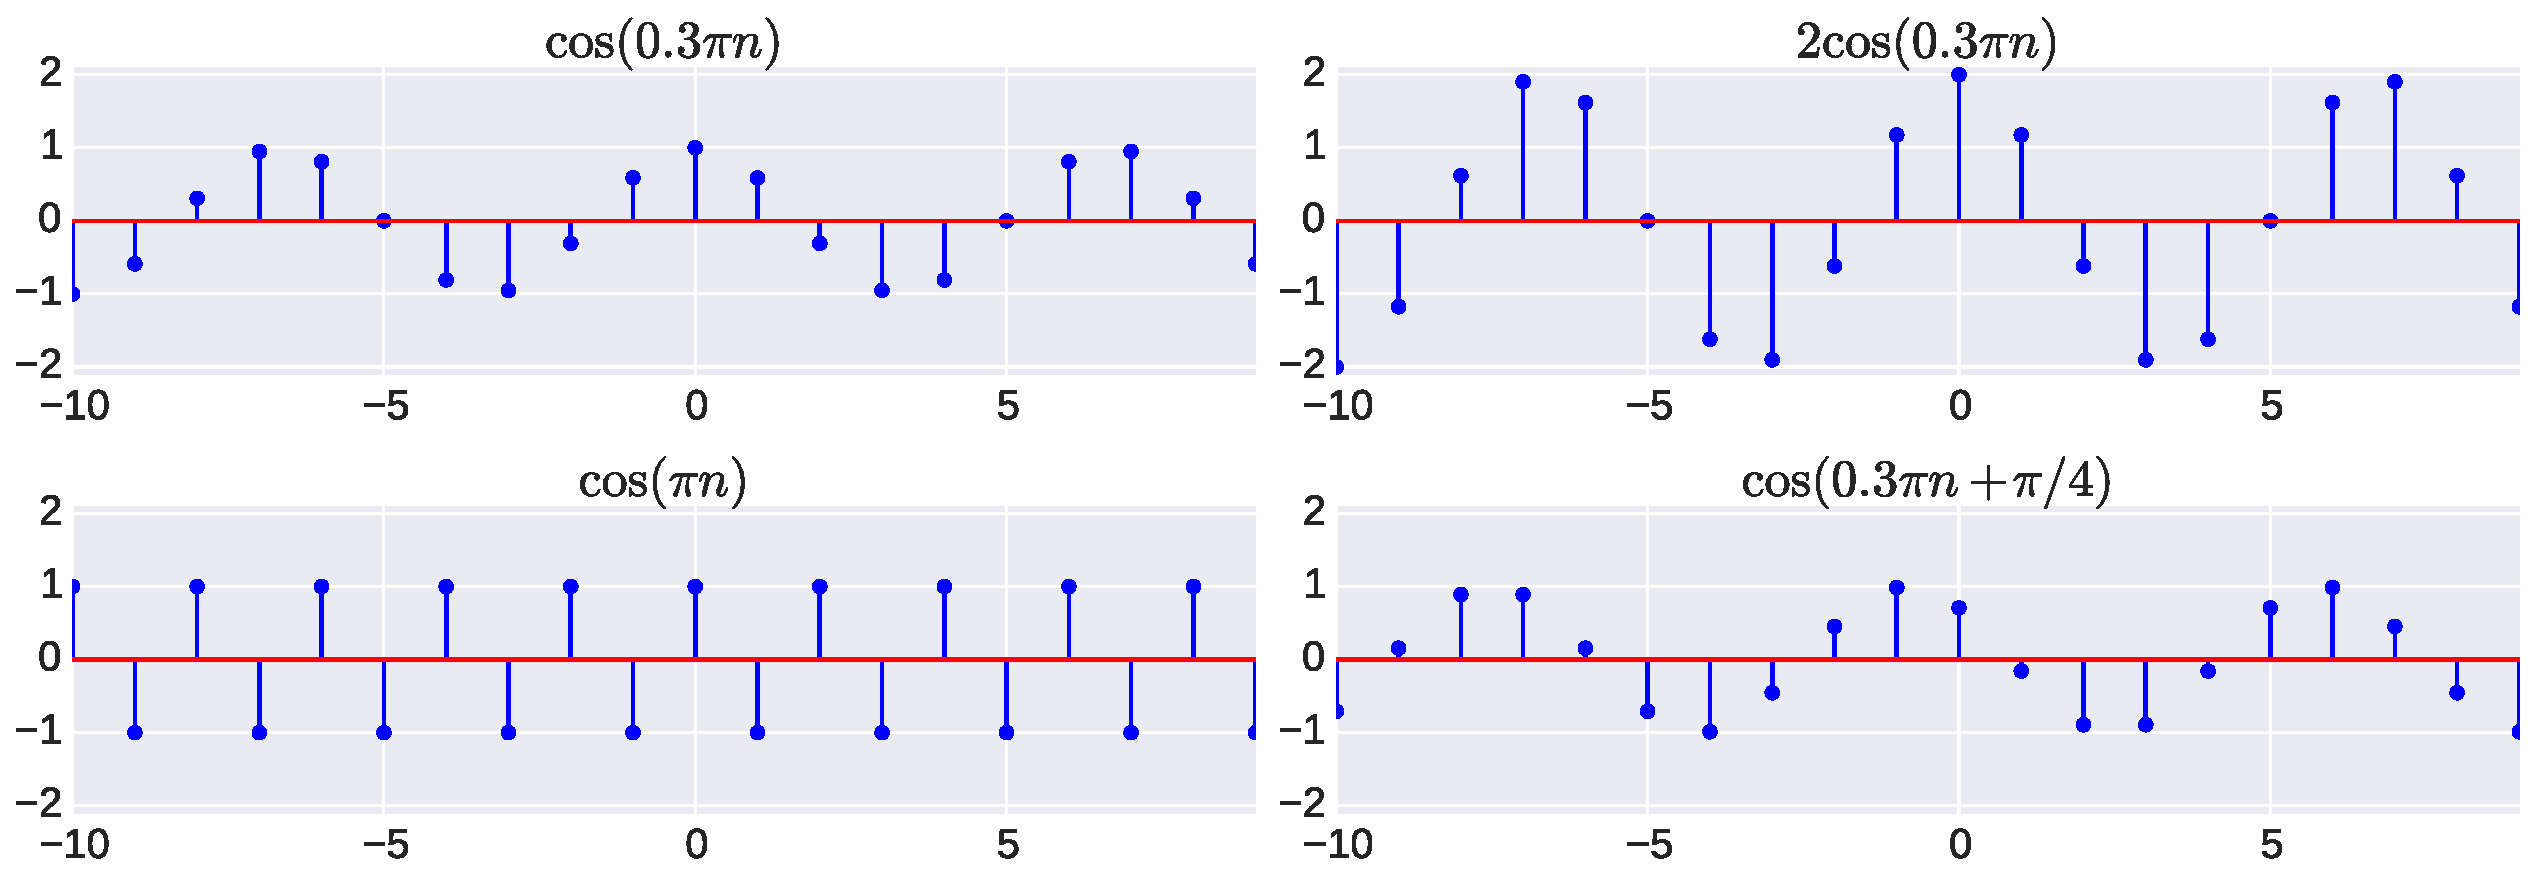
\includegraphics[width=\textwidth]{img/disc_sinu.eps}
\end{figure}

What is the fundamental period?
\end{frame}

% SINUSOIDAL SIGNALS
\begin{frame}[t]{Sinusoidal signals (Contd ...)}

\textbf{There are some peculiarities to the discrete sinusoid:}
\begin{itemize}
\item Not all sinusoids are periodic! e.g. $\sin(n)$
\item There is a maximum frequency for discrete sinusoids. What is it?
\item Two sinusoids that differ by a discrete frequency of $2\pi$ are the same sinusoids.
\end{itemize}

\end{frame}

% SINUSOIDAL SINGALS
\begin{frame}[t]{Sinusoidal signals (Contd ...)}\

\textbf{Complex exponential representation of sinusoids}

\[ z = a + jb = \left|z\right|e^{j\theta} = \left|z\right|\cos \theta + j \left|z\right|\sin \theta\]

\begin{figure}
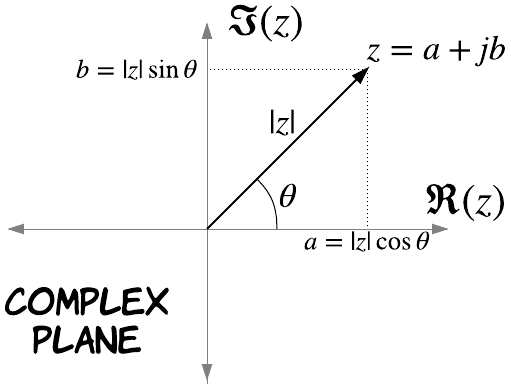
\includegraphics[width=0.5\textwidth]{img/complex_plane.png}
\end{figure}

\[ \cos \theta = \frac{e^{j\theta} + e^{-j\theta}}{2} \,\,\,\,\, \sin \theta = \frac{e^{j\theta} - e^{-j\theta}}{2j}\]

\end{frame}

% EXPONENTIAL SINUSOIDS
\begin{frame}[t]{Exponential sinusoids}
\textbf{Continuous-time} version

Amplitude modulated sinusoids
\[ x[n] = a b^{n} \sin \left(\Omega n + \phi \right), \,\,\,\,\, a, b, \Omega, \phi \in \mathbb{R}\]

\begin{figure}
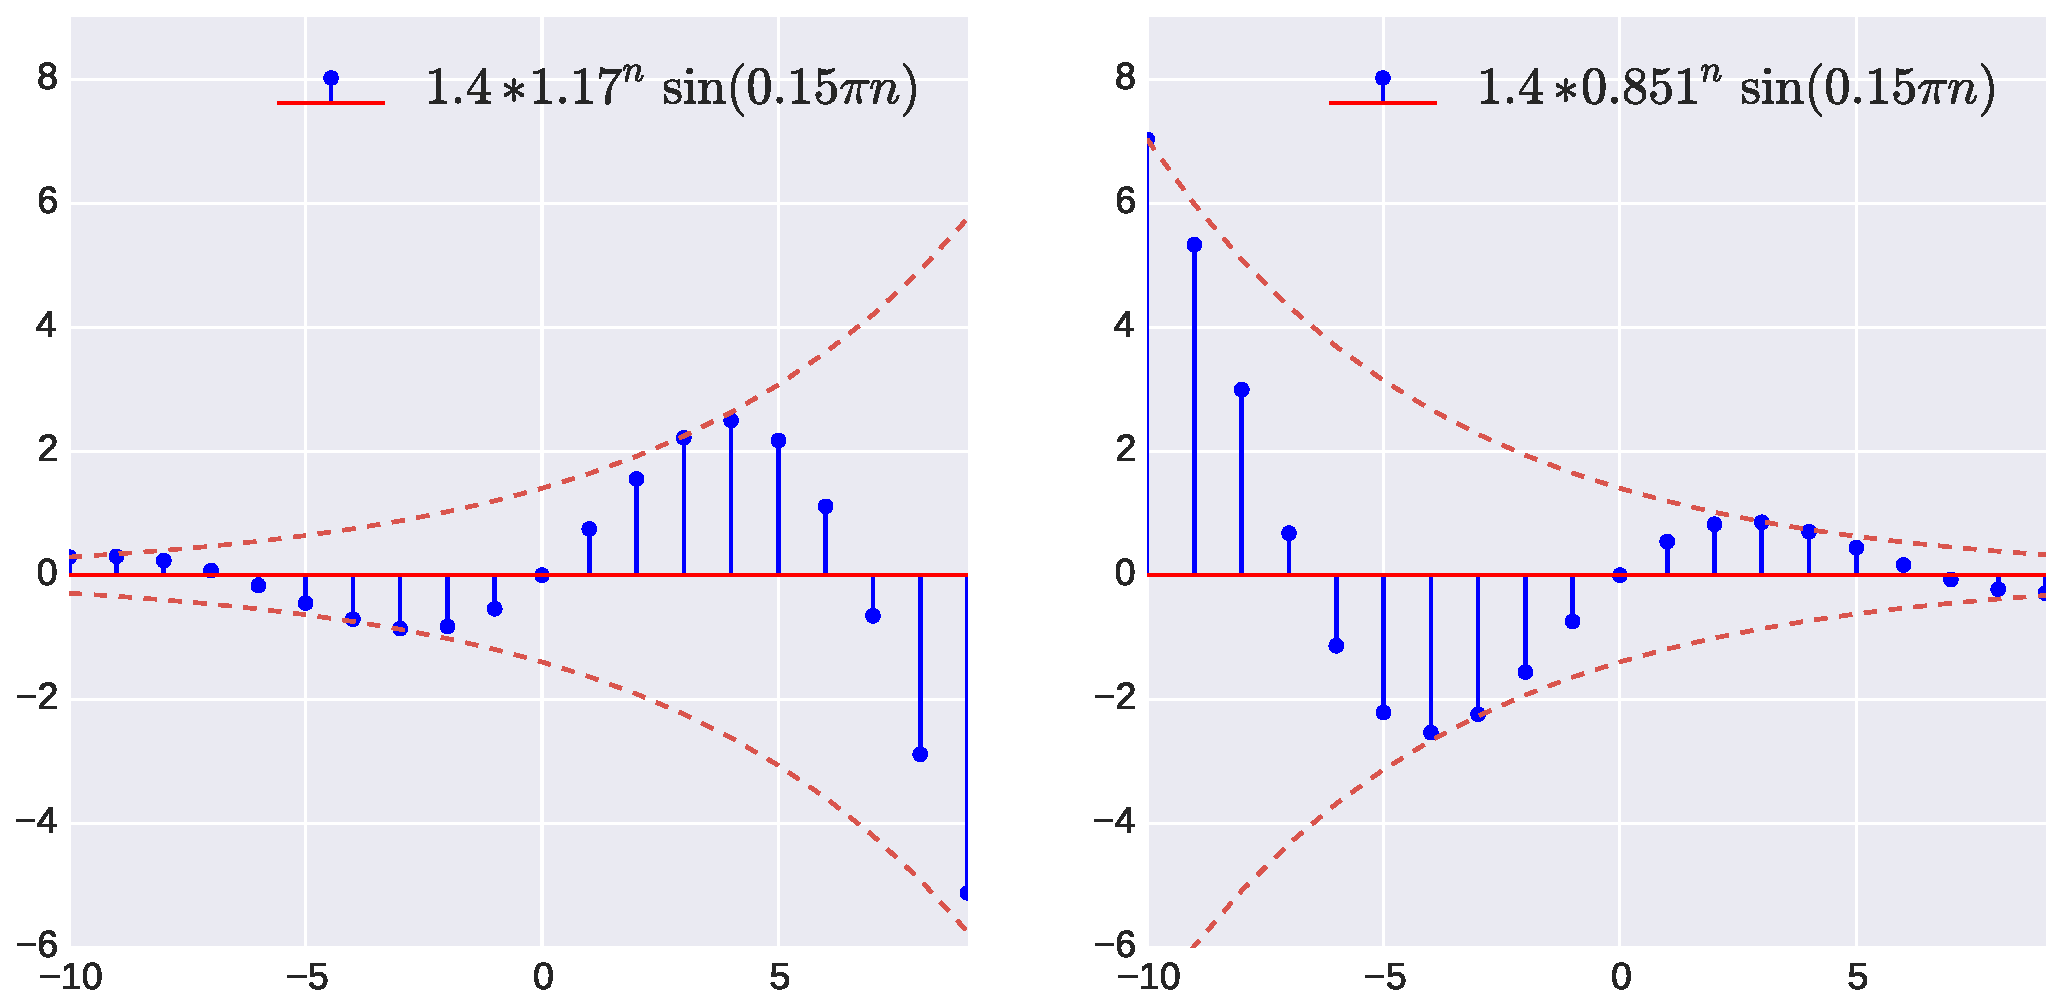
\includegraphics[width=\textwidth]{img/disc_exp_sin.eps}
\end{figure}

\end{frame}

% IMPULSE FUNCTION
%\begin{frame}[t]{Impulse function $\delta(t)$, $\delta[n]$}
%
%\textbf{Dirac delta function} $\delta(t)$
%
%\begin{itemize}
%\item This is \textbf{\underline{NOT}} a conventional function.
%\item It makes sense only when it is used in an integral.
%\item It is not characterized by the exact values it takes as a function of the independent variable, but by the following important property.
%\[ \int_{a}^{b}\delta (t) = \begin{cases}
%1, & 0 \in [a,b] \\
%0, & 0 \notin [a, b]
%\end{cases} \]
%\item It operates like a value selector.
%\[ \int_{-\infty}^{\infty}f(t)\delta (t) = f(0), \text{, where $f$ is continuous at } t= 0. \]
%\item Impulse function is a very useful theoretical tool for representing: point charges or masses, forces in instantaneous collisions, derivatives of jump discontinuities etc.
%\end{itemize}
%\end{frame}
%
%% IMPULSE FUNCTION
%\begin{frame}[t]{Impulse function $\delta(t)$, $\delta[n]$ (Contd ...)}
%
%$\delta(t)$ can be understood through a limiting operation. Let $f_{n}\left(t\right) = \begin{cases}
%n, & -\frac{1}{2n} \leq t \leq \frac{1}{2n} \\
%0, & \mathrm{Otherwise}
%\end{cases}$ and $\int_{-\infty}^{\infty}f_n(t)dt = 1$
%
%\[\int_{-\infty}^{\infty}f_{n}\left(t\right)g\left(t\right)dt = \int_{-\frac{1}{2n}}^{\frac{1}{2n}}ng\left(t\right)dt = g_n \]
%
%\[\lim_{n\to\infty}\int_{-\infty}^{\infty}f_{n}\left(t\right)g\left(t\right)dt = \lim_{n\to\infty}g_{n} = g\left(0\right) = \int_{-\infty}^{\infty}g(t)\delta(t)dt\]
%
%\begin{figure}
%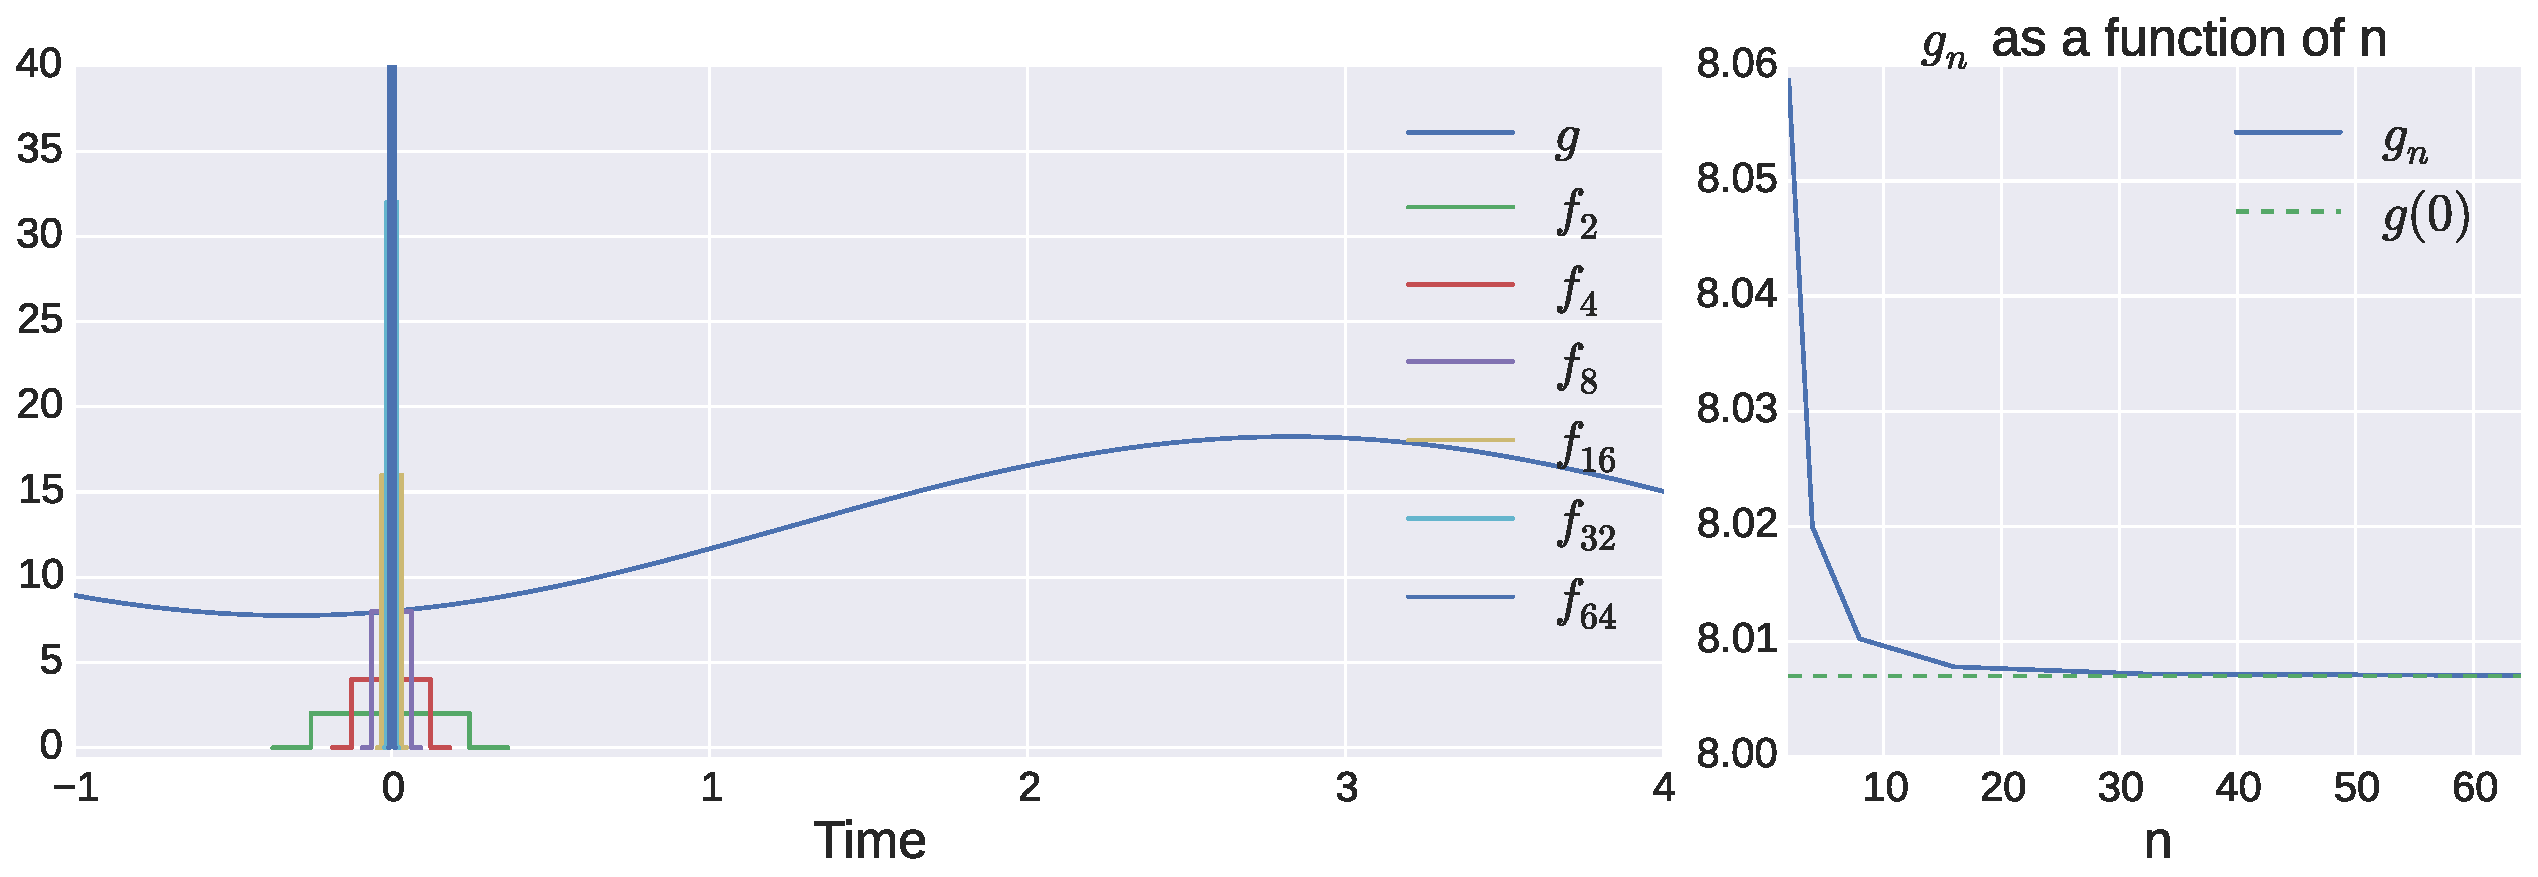
\includegraphics[width=\textwidth]{img/impulse_demo.eps}
%\end{figure}
%\end{frame}

% IMPULSE FUNCTION
\begin{frame}[t]{Impulse function $\delta[n]$}

\textbf{Kronecker delta function or sequence} $\delta[n]$

\begin{itemize}
\item Very easy to understand unlike the continuous-time version.
\[ \delta[n] = \begin{cases}
1 & n = 0 \\
0 & \mathrm{Otherwise}
\end{cases} \]
\end{itemize}

\begin{figure}
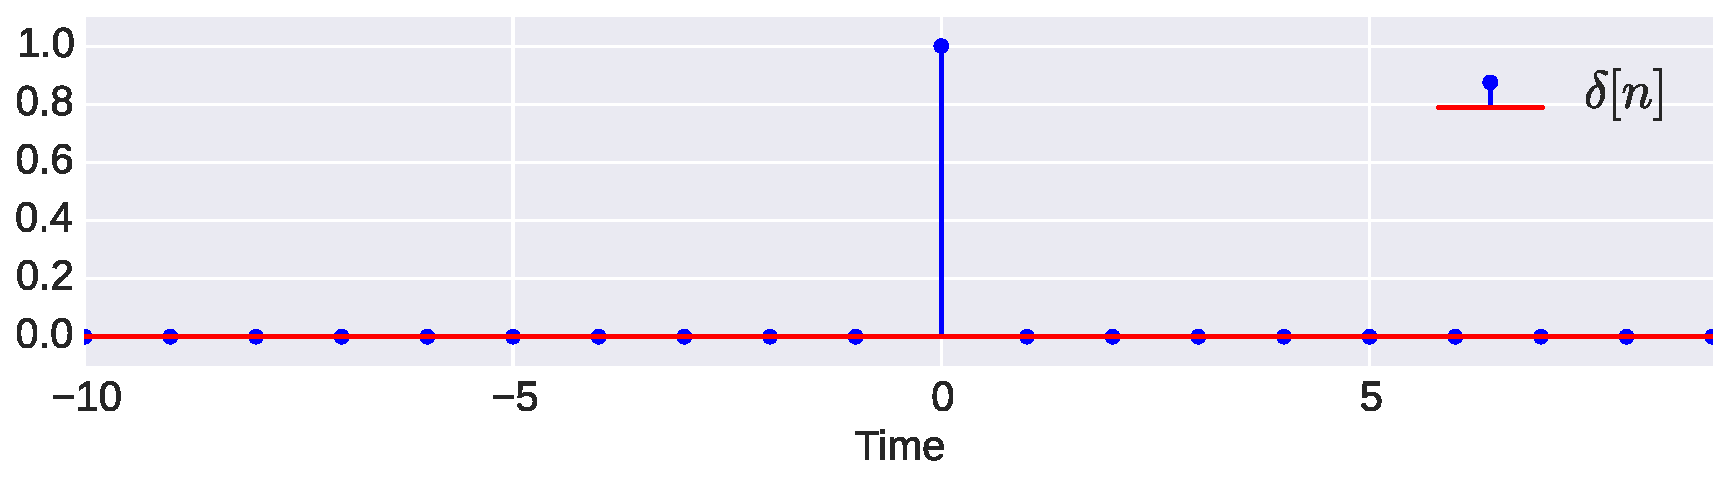
\includegraphics[width=\textwidth]{img/disc_imp.eps}
\end{figure}
\end{frame}

% STEP FUNCTION
\begin{frame}[t]{Step squence $u[n]$}

Definition of \textbf{discrete-time} unit step sequence,
\[ u[t] = \sum_{k=-\infty}^{n} \delta[k] \]

\begin{figure}
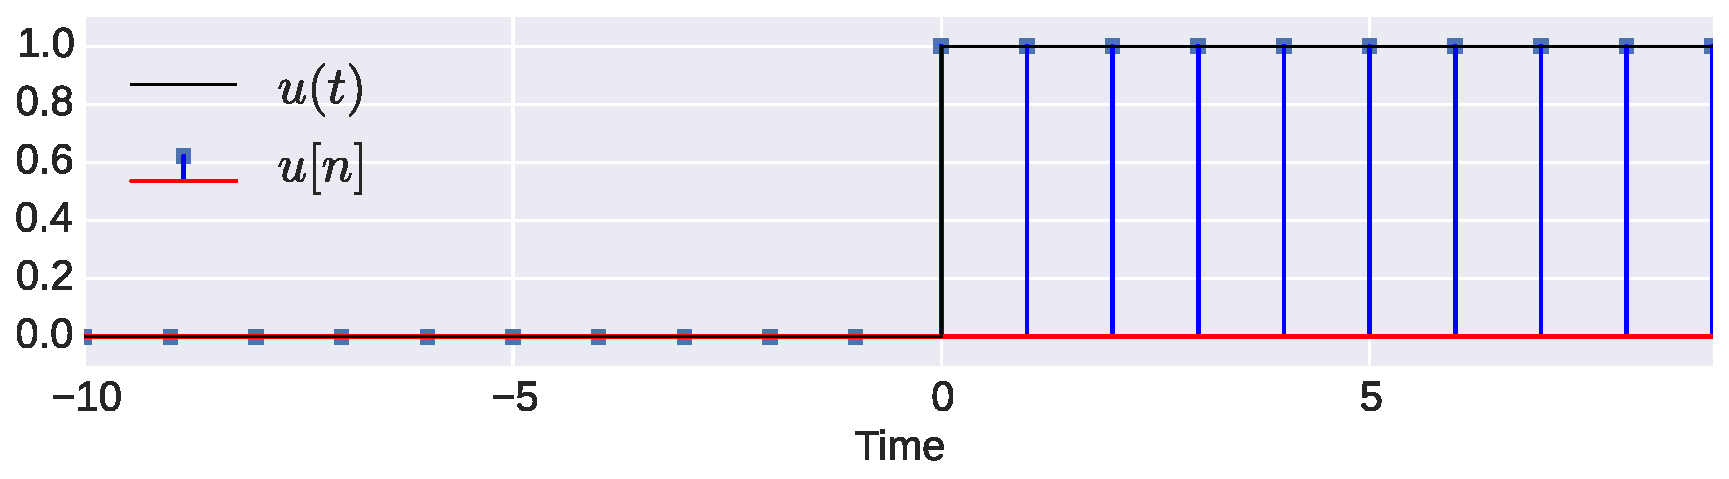
\includegraphics[width=\textwidth]{img/step.eps}
\end{figure}

\end{frame}

\end{document}


